\documentclass{standalone}
\usepackage[utf8]{inputenc}
\usepackage[margin=1in]{geometry}
\usepackage{tikz}
\usetikzlibrary{intersections,positioning}
\tikzset{
    %Define style for boxes
    punkt/.style={
           rectangle,
           rounded corners,
           draw=black, thick,
           text height=.9em,
           text centered},
    % Define arrow style
    pil/.style={
           ->,
           thick,
           shorten <=2pt,
           shorten >=2pt,}
}

\newcommand*{\hnode}[2]{\node[punkt, outer sep=0pt,anchor=base] (#1) {#2\strut};} % create a labelled node
\begin{document}

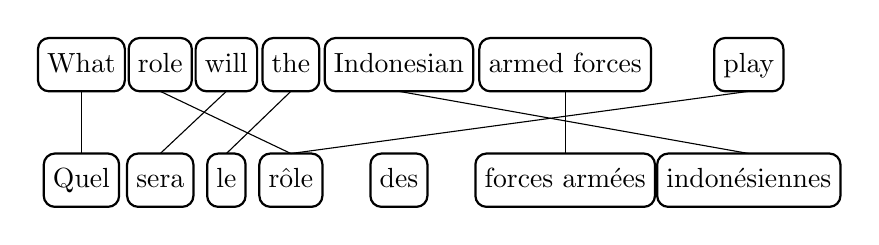
\begin{tikzpicture}
% First make a matrix containing as many columns as the longest sentence.
% Each cell contains a node whose label is identical to the word itself
\matrix[column sep=0em,row sep=.3in] {
% First sentence
\hnode{w1S}{What} & 
\hnode{r2S}{role} & 
\hnode{w3S}{will} & 
\hnode{t4S}{the} & 
\hnode{i5S}{Indonesian} &  
\hnode{a6S}{armed forces}  &
\hnode{p7S}{play}  &
\\

% Now create some dummy nodes to make intermediate nodes
% & & & \node[inner sep={0pt},minimum width=0pt] (p1) {}; & & & \node[inner sep={0pt},minimum width=0pt] (p2) {};\\

% Second sentence
\hnode{q1T}{Quel} & 
\hnode{s2T}{sera} & 
\hnode{l3T}{le} & 
\hnode{r4T}{rôle} & 
\hnode{d5T}{des} & 
\hnode{f6T}{forces armées} & 
\hnode{i7T}{indonésiennes} & 
\\
};

% Now connect the nodes.  For paths that we want to break, name the path
\draw (w1S.south) -- (q1T.north);
\draw (r2S.south) -- (r4T.north);
%\draw[name path=willP] (wS) -- (sT.north);
\draw (w3S.south) -- (s2T.north);
\draw (t4S.south) -- (l3T.north);
\draw (i5S.south) -- (i7T.north);
\draw (a6S.south) -- (f6T.north);
\draw (p7S.south) -- (r4T.north);

% Now break the paths at the intersection by drawing a white circle over it
%\fill[white, name intersections={of=willP and neP}] (intersection-1) circle (4pt);
%\fill[white, name intersections={of=nowP and impP}] (intersection-1) circle (4pt);

% Finally redraw the path you don't want broken
%\draw (p1) -- (nT);
%\draw (iS) -- (p2);
\end{tikzpicture}

\end{document} 